% main.tex
%
% LaTeX template for creating an RASTI paper
%
% v1.4 relased 23 April 2024
%
%
% Copyright (C) Royal Astronomical Society 2024
% Authors:
% Peter Jones (OUP, adapted from mnras_template.tex, author Keith T. Smith (Royal Astronomical Society))

% Change log
%
% v1.0 November 2021
%    Adapted from mnras_template.tex
% v1.1 February 2022
%    rasti.bst updated to match output style for Geophysical Journal International
% v1.2 April 2022
%    minor updates to author instructions (word limit, contact adddress, keywords)
% v1.3 July 2023
%   updated guidance on use of amssymb package
% v1.4 April 2024
%    updated pubyear element to print current year


%%%%%%%%%%%%%%%%%%%%%%%%%%%%%%%%%%%%%%%%%%%%%%%%%%
% Basic setup. Most papers should leave these options alone.
\documentclass[fleqn,usenatbib]{rasti}

% RASTI is set in Times font. If you don't have this installed (most LaTeX
% installations will be fine) or prefer the old Computer Modern fonts, comment
% out the following line
\usepackage{newtxtext,newtxmath}
% Depending on your LaTeX fonts installation, you might get better results with one of these:
%\usepackage{mathptmx}
%\usepackage{txfonts}

% Use vector fonts, so it zooms properly in on-screen viewing software
% Don't change these lines unless you know what you are doing
\usepackage[T1]{fontenc}

% Allow "Thomas van Noord" and "Simon de Laguarde" and alike to be sorted by "N" and "L" etc. in the bibliography.
% Write the name in the bibliography as "\VAN{Noord}{Van}{van} Noord, Thomas"
\DeclareRobustCommand{\VAN}[3]{#2}
\let\VANthebibliography\thebibliography
\def\thebibliography{\DeclareRobustCommand{\VAN}[3]{##3}\VANthebibliography}


%%%%% AUTHORS - PLACE YOUR OWN PACKAGES HERE %%%%%

% Only include extra packages if you really need them. Common packages are:
\usepackage{graphicx}	% Including figure files
\usepackage{amsmath}	% Advanced maths commands
% \usepackage{amssymb}	% Extra maths symbols

%%%%%%%%%%%%%%%%%%%%%%%%%%%%%%%%%%%%%%%%%%%%%%%%%%

%%%%% AUTHORS - PLACE YOUR OWN COMMANDS HERE %%%%%

% Please keep new commands to a minimum, and use \newcommand not \def to avoid
% overwriting existing commands. Example:
%\newcommand{\pcm}{\,cm$^{-2}$}	% per cm-squared

\newcommand{\studentt}[2]{t_\nu \left( #1, #2 \right)}
\newcommand{\depvar}{y_i}
\newcommand{\indepvars}{\boldsymbol{x}_i}
\newcommand{\obsdep}{\hat{y}_i}
\newcommand{\obsindep}{\hat{\boldsymbol{x}}_i}
\newcommand{\indepcov}{\Sigma_{x, i}}
\newcommand{\deperr}{\sigma_{y, i}}
\newcommand{\intscttr}{\sigma_{\text{int}}}
\newcommand{\intercept}{\alpha}
\newcommand{\covariate}{\beta}

%%%%%%%%%%%%%%%%%%%%%%%%%%%%%%%%%%%%%%%%%%%%%%%%%%

%%%%%%%%%%%%%%%%%%% TITLE PAGE %%%%%%%%%%%%%%%%%%%

% Title of the paper, and the short title which is used in the headers.
% Keep the title short and informative.
\title[Robust regression in astronomy]{Robust Bayesian regression in astronomy}

% The list of authors, and the short list which is used in the headers.
% If you need two or more lines of authors, add an extra line using \newauthor
\author[W. Martin \& D. Mortlock]{
William Martin$^{1}$\thanks{E-mail: \href{mailto:w.martin19@imperial.ac.uk}{w.martin19@imperial.ac.uk}}
and Daniel Mortlock$^{1,2}$
\\
% List of institutions
$^{1}$Department of Physics, Imperial College London, Blackett Laboratory, Prince Consort Road, London SW7 2AZ, UK\\
$^{2}$Department of Mathematics, Imperial College London, London, SW7 2AZ, UK
}

% These dates will be filled out by the publisher
\date{Accepted XXX. Received YYY; in original form ZZZ}

% Enter the current year, for the copyright statements etc.
\pubyear{\the\year{}}

% Don't change these lines
\begin{document}
\label{firstpage}
\pagerange{\pageref{firstpage}--\pageref{lastpage}}
\maketitle

% Abstract of the paper
\begin{abstract}
A Bayesian hierarchical model for robust linear regression in the presence of measurement error is described.
The performance of the model is assessed on both simulated and real datasets.
The code is made available for others to use.
\end{abstract}

% Select between one and six entries from the list of approved keywords.
% Don't make up new ones.
\begin{keywords}
methods: statistical -- methods: data analysis -- software: data analysis
\end{keywords}

%%%%%%%%%%%%%%%%%%%%%%%%%%%%%%%%%%%%%%%%%%%%%%%%%%

%%%%%%%%%%%%%%%%% BODY OF PAPER %%%%%%%%%%%%%%%%%%

\section{Introduction}
\label{sec:intro}

% {\color{red}

% (Each point is ~1 paragraph.)

% Regression generally important in astronomy (e.g., M-$\sigma$)

% Astronomy data well characterised errors, but with some outliers

% Previously sigma-clipping or outlier removal; better to model the full measurement process

% Review of previous methods (e.g., Kelly)

% Characterise as an example of robust inference (i.e., don't need to know the actual generating distribution); mention some existing uses of this (e.g., Feeney, Park)

% Then say presenting practical methodology and implementation here.
% }

Linear regression is a common problem in astronomy, arising in fields as
diverse as galaxy formation and evolution (e.g. the black hole
mass -- stellar velocity dispersion correlation --- \citealt{Ferrarese:2000, Gebhardt:2000}), stellar physics (e.g. the
Leavitt law linking the luminosity and pulsation period for Cepheid variable
stars --- \citealt{Leavitt:1912}), and cosmology (e.g. the original formulation of Hubble's law --- \citealt{Hubble:1929}). For this reason, there are a plethora of techniques used by
astronomers for linear regression when both the dependent and independent
variables are measured with error \citep[e.g.][]{Press:1992, Akritas:1996,
Tremaine:2002, Kelly:2007}.

\citet{Kelly:2007} illustrates that common ad-hoc estimators such as
\textsc{fitexy} \citep{Press:1992, Tremaine:2002} and \textsc{bces}
\citep{Akritas:1996} suffer from biases and can underestimate intrinsic scatter.
Similar algorithms exist for removing outliers from data (e.g.\ sigma clipping)
have been used previously but these can lead to controversy (e.g.\ the
reanalysis of the data-set from \citealt{Riess:2011} by \citealt{Efstathiou:2014}). A more principled
approach is to model the entire measurement process.

Bayesian hierarchical models (BHMs) are a natural way to model such datasets ---
these allow astronomers to account for, e.g., measurement errors, selection
effects, interlinked parameters, censored data, and many other effects common to
astronomical problems. BHMs have seen increasing use in astrophysics over the
past few decades, from the distance-redshift relation in cosmology
\citep[e.g.][]{Feeney:2018, Avelino:2019} and photometric redshift estimation
\citep[e.g.][]{Leistedt:2016} to exoplanet characterisation
\citep[e.g.][]{Sestovic:2018} and population-level inference
\citep[e.g.][]{Kelly:2009} --- see \citet{Feigelson:2021} for a recent review
including further examples of BHMs.

\citet{Kelly:2007} presented a general BHM for linear regression with measurement errors and censored data, demonstrating  several advantages
over the other methods considered: no bootstrapping was required to obtain
uncertainties on parameters; the Bayesian approach was easily extensible to
truncated or censored data; and other methods would sometimes severely
underestimate intrinsic scatter in the data. This formulation of Bayesian
regression, sometimes known as \textsc{linmix\_err}, is now commonly used in
astronomy \citep[e.g.][]{McConnell:2013, Bentz:2013, Andrews:2013}.
% However, the model is designed to be sampled using Gibbs sampling, which limits
% the choice of distributions for variables within the model and the number of
% parameters that can be fit simultaneously.
This approach has been extended and refined by others
\citep[e.g.][]{Mantz:2016, Sereno:2016, Bartlett:2023}. These models assume
parameters are normally distributed throughout; however, scientific
uncertainties are often empirically not normally distributed, leading to more
frequent outliers \citep{Bailey:2017}. Inference that relies on normal
distributions can be unduly affected by outliers (see Section \ref{sec:results}
for an exploration of this effect).

The problem of outliers within datasets can be thought of as model
mis-specification: these objects do not fit the distributions used to model them.
The ideas behind robust inference can prove useful for this problem; in robust
inference, methods are designed to work irrespective of the actual generative
distribution \citep{Berger:1994}. One approach is the use of
Student's $t$-distributions, which are leptokurtic (i.e. have heavier tails than
a normal distribution) and can, therefore, lead to more robust results in the
case of model misspecification \citep[e.g.][]{Berger:1994, Gelman:2013}.
Student's $t$-distributions have seen use in bespoke astronomical
\citep[e.g.][]{Park:2017} and cosmological \citep[e.g.][]{Feeney:2018}
inference, but there is not currently a generic robust method for Bayesian
astronomical data analysis.

We propose a development of a generic approach for robust astronomical data
analysis. From the review of previous methods, we can identify properties that
we would like to see in our regression model:

\begin{itemize}
	\item A BHM -- we favour a hierarchical approach
	because it naturally encodes the hierarchical structure of astronomical
	regression problems (i.e.\ objects are drawn from a high-level population;
	the objects intrinsically obey some relationship; the objects are measured
	with error and only the measured values are known). We adopt a Bayesian
	approach both for practical reasons -- the resultant posterior distributions provide full uncertainty quantification -- and due to their logical consistency \citep[e.g.][]{Cox:1946, van_Horn:2003, Knuth:2010}.

	\item A robust model -- we desire a model that is robust to both outliers
	(i.e.\ data points that, whether intrinsically or by virtue of measurement
	errors, do not lie on our regression relation) and model mis-specification
	(i.e.\ where the underlying distribution of data does not match up with the
	distribution assumed for modelling).

	\item A general method -- we seek a model that does not require case-by-case
	optimisation for application to different regression problems (e.g.\ no
	manual outlier identification and removal, no need to rescale prior
	distributions for different problems, etc.).
\end{itemize}

We implement these ideas in this paper, beginning with a discussion of our model
in Section \ref{sec:formalism}. In Section \ref{sec:methods}, we outline the
methods that we use to validate our model; the results of these validation
checks are presented in Section \ref{sec:results}. In Section
\ref{sec:real-world}, we compare the performance of our model on real-world
datasets with the models outlined in \citet{Kelly:2007} and \citet{Park:2017},
before summarising our conclusions in Section \ref{sec:conclusion}.

\section{Formalism}
\label{sec:formalism}

Here we establish notation and set out our model. We
have $N$ astronomical objects, each with some associated independent quantities
$\{\boldsymbol{x}_i\}$ and a dependent quantity $\{y_i\}$. We assume that these
quantities are related by
\begin{align}
    y_i =&\; f(\boldsymbol{x}_i; \boldsymbol{\theta}_f) + \delta_i, \\
    \delta_i \sim&\; \mathcal{P}_{\text{int}} \left( \boldsymbol{\theta}_{\text{int}} \right),
\end{align}
where $f(\boldsymbol{x}_i; \boldsymbol{\theta}_f)$ is a function relating
$\{\boldsymbol{x}_i\}$ to $\{y_i\}$, with parameters $\boldsymbol{\theta}_f$,
and $\mathcal{P}_{\text{int}}$ is an unknown probability distribution with
parameters $\boldsymbol{\theta}_{\text{int}}$.

These objects are then observed, resulting in the measured
data
\begin{align}
    \hat{\boldsymbol{x}}_i =&\; \boldsymbol{x}_i + \boldsymbol{\epsilon}_{x,i}, \\
    \hat{y}_i =&\; y_i + \epsilon_{y,i}, \\
    \boldsymbol{\epsilon}_{x,i} \sim&\; \mathcal{P}_{\text{obs}} \left( \boldsymbol{\theta}_{\text{obs}} \right), \\
    \epsilon_{y,i} \sim&\; \mathcal{P}_{\text{obs}} \left( \boldsymbol{\theta}_{\text{obs}} \right),
\end{align}
where $\mathcal{P}_{\text{obs}}$ is an unknown probability distribution with
parameters $\boldsymbol{\theta}_{\text{obs}}$.

In a Bayesian framework, we can extend this model to deal with, e.g., censored
data or selection effects, but this is beyond the scope of the current work ---
see \citet{Kelly:2007} for an overview of an approach that would incorporate
these effects.

\subsection{Building a robust model}
\label{sec:formalism.robust}

In the setup outlined above, the form of the distributions
$\mathcal{P}_{\text{int}}$ and
$\mathcal{P}_{\text{obs}}$ are unknown. A common
assumption in analysis is to use normal distributions to model both of these
distributions. However, in the case of model mis-specification (where, e.g., we
assume $\mathcal{P}_{\text{int}}$ is a normal distribution but it is a different
distribution), the results obtained under this assumption can be biased.
Making the assumption that $\mathcal{P}_{\text{int}}$ follows a different
distribution, such as a Student's $t$-distribution \citep{Andrews:1974} or a Gaussian
mixture model \citep{Aitkin:1980}, can give results that are robust to this model
misspecification. This means that, even though we do not believe that the
distribution we choose to model $\mathcal{P}_{\text{int}}$ is the same as the
underlying, unknown $\mathcal{P}_{\text{int}}$, we can be confident in the
inferences about the regression model and the properties of individual objects.

In this paper, we use Student's $t$-distributions to build a model that is
robust to model misspecification.

\subsection{Sampling distribution}
\label{sec:formalism.sampling}

For robust inference, we seek a sampling distribution that can have heavier
tails than a normal distribution, but that can reduce to a normal distribution
when the underlying dataset is normally distributed. We further seek an
identifiable model, and a differentiable distribution which can be fit using
Hamiltonian Monte Carlo (HMC). These constraints lead us naturally to Student's
$t$-distributions, which fulfil all of these criteria.

Student's $t$-distributions are encountered when estimating the mean of a normal
distribution with unknown variance from a limited number of samples. The number
of samples is a parameter of the distribution: for $n$ samples, the
corresponding Student's $t$-distribution will have $\nu \equiv n - 1$
``degrees-of-freedom''. This value of $\nu$ parameterizes how heavy-tailed the
distribution is. While the interpretation of $\nu$ as ``degrees-of-freedom''
only makes sense for $\nu \in \mathbb Z^+$, the distribution is normalizable for
any positive, real $\nu$; for this reason, we shall refer to $\nu$ as the shape
parameter.
% Constructing a statistical model that treats this shape parameter as
% a free parameter to be fitted allows the model to adapt to outliers in the data,
% reverting to the result of a model that uses normal distributions in the absence
% of outliers \citep{Feeney:2018}. In this context, $\nu$ is considered a
% nuisance parameter: its exact value is unimportant, and its inclusion in the
% model is solely to ensure that inference is robust to outliers.

The Student's $t$-distribution, with location $\mu$ and scale $\sigma$, has
the probability density function
\begin{equation}
    t_{\nu} \left(x; {\mu}, {\sigma}\right)
        =
    \frac{1}{\sqrt{\pi \nu} \sigma}
    \frac{
        \Gamma \left(\frac{\nu + 1}2\right)
    }{
        \Gamma \left(\frac{\nu}2\right)
    }
    \left(
        1 + \frac{1}{\nu} \frac{\left(x - \mu\right)^2}{\sigma^2}
    \right)^{
        -\frac{\nu + 1}{2}
    }.
\end{equation}
This is shown for a range of $\nu$ in Figure \ref{fig:model.t}: $\nu
= 1$ gives a Cauchy distribution; and $\nu \rightarrow \infty$ tends to a normal
distribution. The distribution has mean
\begin{equation}
    \mathbb{E}(x)
        =
    \begin{cases}
        \mu & \nu > 1, \\
        \textrm{undefined} & \textrm{otherwise}
    \end{cases}
\end{equation}
and variance
\begin{equation}
    \mathrm{Var}(x)
        =
    \begin{cases}
        \frac{\nu}{\nu - 2} \sigma^2 & \nu > 1, \\
        \infty & 1 < \nu \leq 2, \\
        \textrm{undefined} & \textrm{otherwise.}
    \end{cases}
\end{equation}

\begin{figure}
	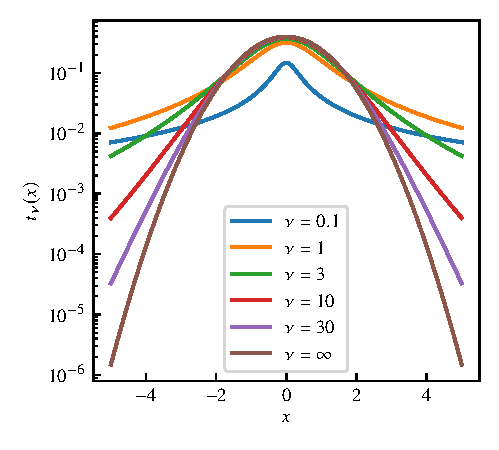
\includegraphics{graphics/t-dist-log.pdf}
    \caption{The $t$-distribution probability density function for different
    values of shape parameter, $\nu$.}
    \label{fig:model.t}
\end{figure}

In this paper, we have found it useful to define two quantities for comparison
with normal distributions. The first, $\sigma_{68}(\nu)$, is the width of the
highest density interval for a $t$-distribution with scale parameter
$\sigma = 1$ such that the density contained in the interval is equal to that
of a 1$\sigma$ interval for a normal distribution. This is given by
\begin{equation}
    \sigma_{68}(\nu) =
        \sqrt{
            \nu \left(
                \frac{1}{I^{-1}(\Phi_{\sigma=1};\frac\nu2, \frac12)} - 1
            \right)
        },
\end{equation}
where $\Phi_{\sigma=1} = \text{erf}\left(\frac{\sqrt{2}}2\right) \approx 0.6827$
is the posterior density contained within $\pm1\sigma$ of the mean for a normal
distribution, and $I^{-1}$ is the inverse of the regularized incomplete beta function, which we define as
\begin{equation}
    I(x; a, b) = \frac{
        \int_0^x t^{a-1} (1 - t)^{b-1} {\rm d}t
    }{
        \int_0^1 t^{a-1} (1 - t)^{b-1} {\rm d}t
    }
\end{equation}
This quantity is useful for defining a ``scale'' parameter that is less tightly
coupled to $\nu$ than the $\sigma$ parameter of the $t$-distribution.

The second quantity we use is an ``outlier fraction'' $\omega$, which
is defined as the fraction of points expected to lie more than $3\sigma$ from the
distribution mean $\mu$. For a $t$ distribution, this is given by
\begin{eqnarray}
    \omega(\nu)
    &=& P\left(
        \left|x - \mu \right| > 3 \sigma \;
        \middle| \;
        x \sim \studentt{\mu}{\sigma}
    \right) \label{eqn:model.outlier_frac}\\
    &=& 2 F_\nu \left(\mu - 3 \sigma \right),
\end{eqnarray}
where $F_\nu(x)$ is the cumulative distribution function for the Student's
$t$-distribution with shape parameter $\nu$. Figure \ref{fig:model.outlier_frac}
shows the relationship between outlier fraction $\omega$ and shape parameter
$\nu$, with $\omega \rightarrow 2.70 \times 10^{-3} $ in the limit of a normal
distribution, i.e., as $\nu \rightarrow \infty$.  Under this definition
approximately 1 in 370 data-points would be outliers for data that follows a
normal distribution; for Cauchy-distributed data (i.e. $\nu = 1$), every fifth
data-point to be an outlier.

\begin{figure}
	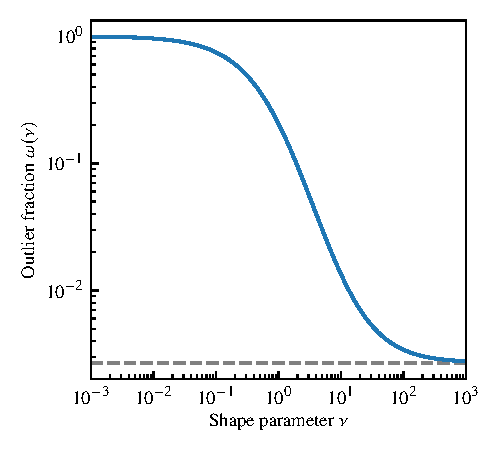
\includegraphics{graphics/outlier_frac.pdf}
    \caption{The outlier fraction, $\omega$, for different values of shape
    parameter, $\nu$. The outlier fraction of a normal distribution ($\approx
    2.70 \times 10^{-3}$) is indicated by the dashed grey line.}
    \label{fig:model.outlier_frac}
\end{figure}

\subsection{Regression model}
\label{sec:formalism.model}

Our regression model, represented as a directed acyclic graph in
Figure~\ref{fig:formalism.dag}, is specified here. We assume a linear
relationship between
$\{\boldsymbol{x}_i\}$ and $\{y_i\}$, i.e.
\begin{equation}
    f(\boldsymbol{x}_i; \boldsymbol{\theta}_f) =
        \alpha + \boldsymbol{\beta} \cdot \boldsymbol{x}_i
\end{equation}
where $\{\alpha, \boldsymbol{\beta}\} \equiv \boldsymbol{\theta}_f$. In this
paper, we only consider this linear relationship, but this apparatus could be
used for other, non-linear relationships between variables with different
parameters.

Similarly to \citet{Kelly:2007}, we define a Bayesian hierarchical model to
reflect the nature of the regression problem. Firstly, we assume that we can
represent the probability distribution $\mathcal P_{\text{int}}$ with a
Student's $t$-distribution with shape parameter $\nu$ and scale parameter
$\sigma_{\text{int}}$ --- i.e.
\begin{equation}
\depvar \sim \studentt{\intercept + \covariate \indepvars}{\intscttr}.
\end{equation}
We use a Student's $t$-distribution here not because we believe that the data
intrinsically follows this distribution, but because the resulting model is
robust to model mis-specification --- such as if a galaxy were
to be an outlier from a particular relation as a result of a recent merger.

We assume that we can represent the probability distribution
$\mathcal P_{\text{obs}}$ as a normal distribution with scale parameter given by
the error associated with the measured quantity. These measurements are modelled
as
\begin{align}
    \obsindep \sim&\; \mathcal N\left({\indepvars}, \indepcov^2\right) \\
    \obsdep \sim&\; \mathcal N\left({\indepvars}, \deperr^2\right).
\end{align}

We experimented with assuming $\mathcal P_{\text{obs}}$ to be $t$-distributed,
but found that the resultant model was difficult to sample as a result of its
geometry, and that posterior predictive checks often included large outliers and
did not resemble the datasets that gave rise to them.  Fortunately, for robust
inference the presence of a single heavy-tailed component is sufficient.

This model structure is represented as a directed acyclic graph in Figure
\ref{fig:formalism.dag}.

\begin{figure}
	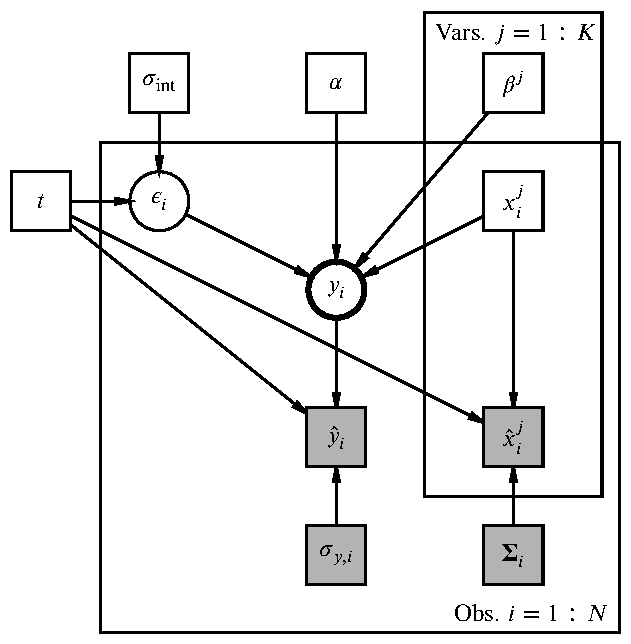
\includegraphics[width=\columnwidth]{graphics/dag.pdf}
    \caption{A directed acyclic graph representing the $t$-cup model for the
    function $f(\boldsymbol{x}; \boldsymbol{\theta}) = \alpha +
    \boldsymbol{\beta} \cdot \boldsymbol{x}_i$.}
    \label{fig:formalism.dag}
\end{figure}

\subsection{Priors}
\label{sec:formalism.prior}

To ensure that our model is generically applicable to astronomical linear
regression, we ensure that both independent and dependent quantities are scaled
to have zero mean and unit variance. This allows us to set generic priors on the
scaled intercept, gradients and scatter $\{\tilde{\intercept},
\tilde{\covariate}, \tilde{\sigma}_{\text{int}}\}$ that do not require rescaling
for different units or datasets (though these priors can be revised to
incorporate prior information).

Our default priors on the regression parameters $\{\tilde{\intercept},
\tilde{\covariate}, \tilde{\sigma}_{\text{int}}\}$ are
\begin{align}
    \tilde{\intercept} \sim&\; \mathcal N(\mu = 0, \sigma = 2), \\
    \tilde{\covariate} \sim&\; \mathcal N(\mu = 0, \sigma = 2), \\
    \tilde{\sigma}_{68} \sim&\; \Gamma(1.1, 5).
\end{align}
The motivation behind the prior on $\tilde{\intercept}$ is that, as the data is
pre-scaled to have zero mean and the relationship between quantities is assumed
to be linear, we would expect the data to have zero intercept. Similarly, the
prior on $\tilde{\beta}$ has been chosen because the pre-scaling of the data
suggests a gradient between $-1$ and $1$. The prior on $\tilde{\sigma}_{68}$ is
informed by \citet{Chung:2013}, who demonstrate that a prior with density at
$\tilde{\sigma}_{\text{int}} = 0$ will lead to a prediction of no intrinsic
scatter in datasets where intrinsic scatter is present; in addition, there is a
reasonable physical argument that most astrophysical processes will not produce
objects with no population scatter. The chosen prior balances this constraint
with difficulties arising in testing as a result of the pre-scaling, which led
to insufficient prior density at small levels of intrinsic scatter.

The prior on the latent values of the independent quantities $\{\indepvars\}$ is
a Gaussian mixture model prior, similar to that used in \citet{Kelly:2007}.
While \citeauthor{Kelly:2007} infers the complete prior as part of the model, we
found that such a prior led to sampling issues as a result of the lack of
identifiability inherent in a multicomponent Gaussian mixture model. Therefore,
we use extreme deconvolution \citep{Bovy:2011} to estimate the parameters of a
Gaussian mixture model approximating the latent distribution of
$\{\indepvars\}$, and use these parameters for the prior.

The prior on the shape parameter $\nu$ is
\begin{align}
    \nu \sim&\; \text{Inv-}\Gamma(4, 15);
\end{align}
this prior was chosen to balance flexibility (such that the model could
accommodate both heavily leptokurtic distributions --- e.g. the Cauchy
distribution --- and normally-distributed data) and sampling issues (as $\nu
\leftarrow \infty$, different values of $\nu$ become rapidly indistinguishable).
The reasoning behind this choice of prior is expanded upon in Appendix
\ref{sec:t-prior}. The exact choice of prior for $\nu$ is unimportant, as the
model is designed to be robust to model mis-specification; the only key element
is that $\nu$ is allowed to vary to accommodate both normal and heavy-tailed
distributions. By virtue of this, difficulties in sampling $\nu$ according to
this prior distribution do not invalidate the results of the model, as long as
there is coverage at both small and large values of $\nu$.

\subsection{Asymptotic normality}
\label{sec:formalism.asymptotic}

One potential disadvantage of adopting a heavy-tailed likelihood in the
statistical model is that the resultant inferences would, in general, be less
constraining than under the assumption of a normal model (see, e.g., the
motivation behind the mixture model proposed in \citealt{Tak:2019}).  If there
are no outliers, the implication would be that the robust approach is inferior.

This effect would be appreciable for the smallest datasets -- the posteriors
would have heavier tails than under a normal model -- but, in this case,
meaningful constraints are unlikely irrespective of the adopted model. For
larger datasets, of more than a few tens of points, these tails are effectively
multiplied out, typically leaving just a single region of high probability.
Moreover, for the regression problem considered here, the posterior in the
regression parameters satisfies the requirements for asymptotic normality
\citep[e.g.][]{Ghosh_etal:2006}, so the core of the posterior is Gaussian in
form, just as would be the case under a normal model.  (There is not even a
significant numerical cost as the posterior has to be evaluated by sampling
anyway.)

{\color{red} Discuss figure \ref{fig:formalism.posterior-sd}}

\begin{figure}
    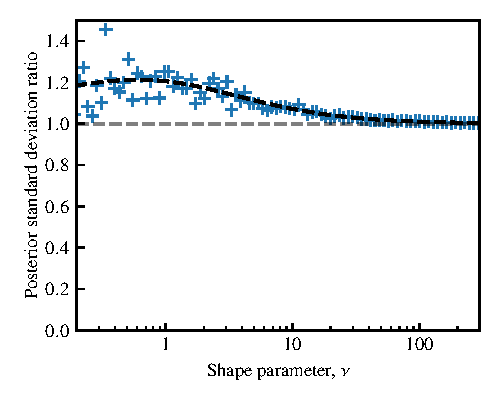
\includegraphics[width=\columnwidth]{graphics/posterior_sd.pdf}
    \caption{}
    \label{fig:formalism.posterior-sd}
\end{figure}

{\color{blue} I don't know whether it's worth discussing \citet{Tak:2019} in
this section, and the reason for not adopting their approach (a mixture model
with a $t$ component)? They say that their approach is better than a single $t$
distribution --- ``A heavy tailed error assumption based on Student’s t
distribution helps reduce the bias. However, it may be less efficient in
estimating parameters if the heavy tailed assumption is uniformly applied to all
of the data when most of them are normally observed''... I've added a
parenthetical comment to incorporate this}

\subsection{Implementation}
\label{sec:formalism.implementation}

The model described in Section \ref{sec:formalism.model} is implemented in
NumPyro \citep{NumPyro, Pyro}, which is used to draw samples via a HMC No U-Turn
Sampler. The implementation is packaged as $t$-cup, available as a Python
package\footnotemark.

For the purposes of comparison, we have also implemented a model that mirrors
the above structure, but uses normal distributions at each stage --- we refer to
this as $n$-cup.

\footnotetext{\url{https://github.com/wm1995/tcup}}

\section{Validation}
\label{sec:methods}

In this section, we outline the methods used to validate the model set out in
Section~\ref{sec:formalism}. We run two types of tests to validate the performance of
$t$-cup under different types of model mis-specification: simulation-based
calibration tests \citep{Cook:2006, Talts:2018}; and fixed value calibration
tests.

\subsection{Simulation-based calibration}
\label{sec:methods.sbc}

Simulation-based calibration tests \citep{Cook:2006, Talts:2018} are used to
diagnose sampling issues. Parameters of interest $\theta_0$ are drawn from the
model prior $\pi(\theta)$, and a dataset is drawn following the prescription of
the model. We can then run a single MCMC chain on this dataset until we have
drawn $L$ independent samples $\{\tilde{\theta}_{i}\}$ (see \citet{Talts:2018}
for a discussion of independence criteria). We then compute the rank statistic
\begin{equation}
    r(\theta_0, \tilde{\boldsymbol{\theta}}_{\text{MCMC}})
        = \sum_{i = 1}^{L} \mathbb I (\tilde{\theta}_i < \theta_0),
\end{equation}
where $\mathbb{I}(\cdot)$ is the indicator function which evaluates to 1 if its (logical) argument is true and 0 if it is false.
If the generative model matches the sampling model and the sampling algorithm
correctly draws from the posterior, the rank statistic will be uniformly
distributed across the integers $[0, L]$. We can, therefore, repeat this process
many times to build a histogram of rank statistics; any shortfalls in the
sampling algorithm will manifest as deviations from uniformity.

While this procedure has been developed to diagnose sampling issues, we can also
use the method to build a heuristic measure of how robust a model is to
mis-specification. If the generative model and the sampling model no longer
match, we would expect deviations from uniformity in the rank statistic
histogram. We can compare how well different sampling models deal with model
mis-specifcation by building the rank statistic histogram and assessing the
deviation from uniformity.

As our priors are defined in a scaled space, our simulation-based calibration
tests are also conducted in this scaled space; in this way, we are solely
testing the performance of the MCMC models, and not of the scaling before
fitting the models.

\subsection{Fixed-value calibration}
\label{sec:methods.fixed}

For our fixed-value calibration tests, we simulate datasets from known models
with true fixed values for our regression parameters. The purpose of these tests
is to demonstrate accurate recovery of these values, and to compare with the
results given when using normal distributions.

We generate multiple datasets with the same ground-truth parameters to verify
the results across multiple runs, producing plots of the composite cumulative
distribution function across each dataset. In each instance, full specifications
of the data models are given in Appendix \ref{sec:data-models}.

We aim to do a full end-to-end test of our inference pipeline in the fixed-value
calibration tests; therefore, these datasets are generated in the unscaled space
and are a test not only of the sampler but also of the scaling.

\section{Results on simulated datasets}
\label{sec:results}

In the previous section, we proposed a general-purpose, robust statistical model
for linear regression; in this section, we investigate the performance of the
model on a series of simulated datasets with known parameters. Code that
reproduces the datasets in this section is available online\footnotemark.

\footnotetext{\url{https://github.com/wm1995/tcup-paper}}

\subsection{\textit{t}-distributed data}
\label{sec:results.t}

\begin{figure*}
    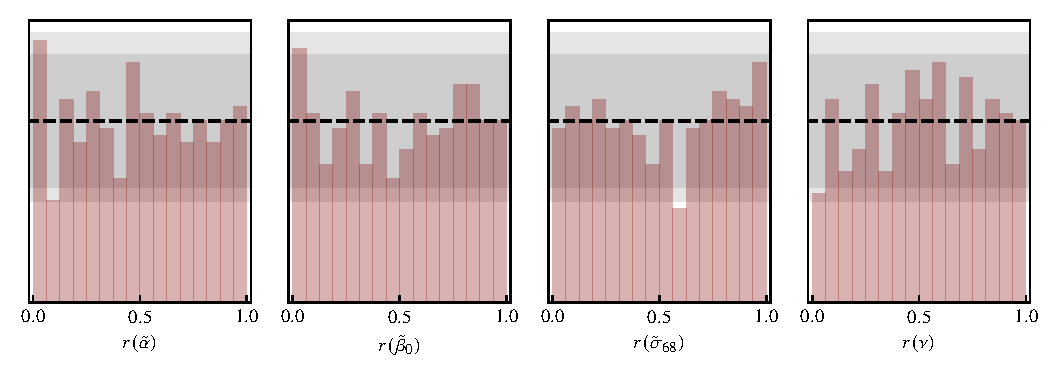
\includegraphics[width=\textwidth]{graphics/sbc/tcup_sbc.pdf}
    \caption{SBC runs for the t distribution under $t$-cup. If the inference
    procedure is working as expected, the histograms for each parameter should
    be distributed uniformly (as indicated by the black dashed line). The dark
    (light) grey regions correspond to the 94\% (98\%) confidence interval of
    uniformity (i.e.\ we expect one histogram bin per panel (figure) to lie
    outside of this range).}
    \label{fig:results.t.sbc}
\end{figure*}

For our first test, we start with a dataset that matches our model perfectly
(i.e.\ $\mathcal P_{\text{int}} = t_\nu, \mathcal P_{\text{obs}} = \mathcal{N}$).
The simulation-based calibration tests indicate that the rank statistic is
consistent with being uniformly distributed (see Figure
\ref{fig:results.t.sbc}), and, therefore, that our inference procedure is
working as expected.

For our fixed-value tests, we drew $N = 20$ datapoints with $(\alpha, \beta,
\sigma_{68}, \nu) = (3, 2, 0.1, 3)$; the full model used to generate the data is
specified in Appendix \ref{sec:data-models.t}. The chosen value of $\nu = 3$
corresponds to an outlier fraction of $\omega(\nu = 3) \approx 5.8 \%$.  As
shown in Figure \ref{fig:results.t.corner}, we recover the values of the
parameters that were used to generate the dataset; these values are consistent
with a model where the shape parameter is fixed to $\nu = 3$.

\begin{figure}
    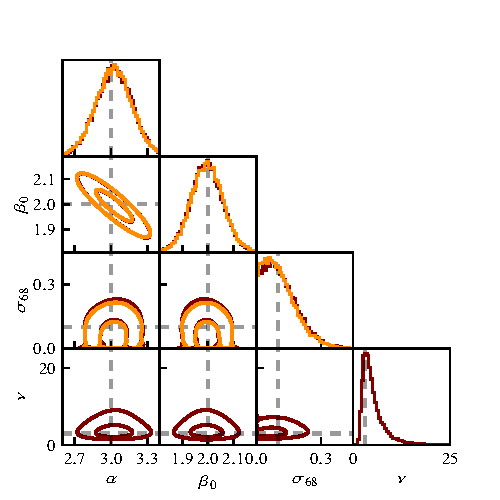
\includegraphics[width=\columnwidth]{graphics/fixed/corner_t.pdf}
    \caption{The posterior for each of the regression coefficients and the shape
    parameter $\nu$ for the \textit{t}-distributed dataset, with ground-truth
    values indicated by the black dashed lines. Contours indicate 39.3\% and
    86.5\% highest posterior density regions, corresponding to 1$\sigma$ and
    2$\sigma$ contours for a bivariate normal distribution.}
    \label{fig:results.t.corner}
\end{figure}

We then generated 400 datasets from the same ground-truth parameters, and ran
MCMC against each dataset.
% We combined samples from each of the MCMC runs to produce a plot of the
% cumulative distribution function for the regression coefficients and shape
% parameter $\nu$. The results shown in Figure \ref{fig:results.t.map} indicate
% that the estimate of true parameter values is unbiased.
95\% highest posterior density credible intervals were constructed for each run;
the true parameter values were contained in these credible intervals $97\%$,
$96\%$ and $98\%$ of the time for the intercept $\alpha$, the slope $\beta$ and
the intrinsic scatter $\sigma_{68}$. For the nuisance parameter $\nu$, the
credible intervals contained the true parameter value across all runs; this may
be caused by this parameter being only weakly constrained for these datasets.

\subsection{Normally-distributed data}
\label{sec:results.outlier}

In this test, we compare $t$-cup with an equivalent model that employs normal
distributions to check that:
\begin{enumerate}
    \item $t$-cup is reduces to a normal model in the absence of outliers
    \item $t$-cup gives less biased results when an extreme outlier is present.
\end{enumerate}

We conducted a simulation-based calibration test, where datasets were generated
using normal distributions throughout (i.e.\ $\mathcal P_{\text{int}} = \mathcal
P_{\text{obs}} = \mathcal{N}$). The results (shown in Figure
\ref{fig:results.outlier.sbc}) indicate that, while the estimates of the
intercept and slope are significantly biased when analysed by the normal model
(as indicated by the rank statistic's distribution deviating from normal), the
estimates derived by $t$-cup are unbiased. Additionally, while both $n$-cup and
$t$-cup systematically overestimate the intrinsic scatter $\sigma_{68}$, the
bias is much smaller for $t$-cup than for $n$-cup.


\begin{figure*}
    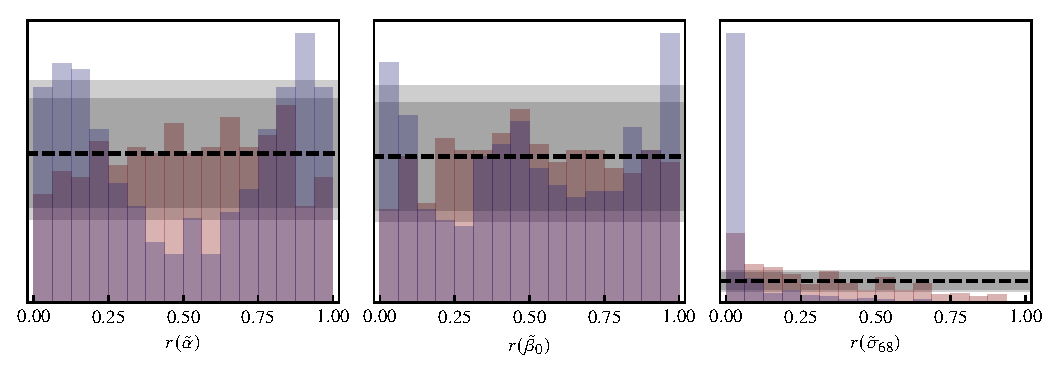
\includegraphics[width=\textwidth]{graphics/sbc/outlier20_sbc.pdf}
    \caption{A rank statistic histogram for 400 simulation-based calibration
    runs for the outlier dataset under $n$-cup (blue) and $t$-cup (red). If
    there were a perfect match between the generative model and the inference
    model, the histograms for each parameter will be distributed uniformly (as
    indicated by the black dashed line). The dark (light) grey regions
    correspond to the 94\% (98\%) confidence interval of uniformity (i.e.\ we
    expect one histogram bin per panel (figure) to lie outside of this range).}
    \label{fig:results.outlier.sbc}
\end{figure*}

A dataset of $N = 12$ points was generated with $(\alpha, \beta, \sigma_{\rm
int}) = (3, 2, 0.2)$, and one of the points was modified to be a
$\sim20\,\sigma$ outlier (the full generative model is given in Appendix
\ref{sec:data-models.outlier}). While such an extreme outlier could easily be
identified and removed, the purpose here is to demonstrate that $t$-cup does not
require this to obtain sensible inferences.

\begin{figure*}
    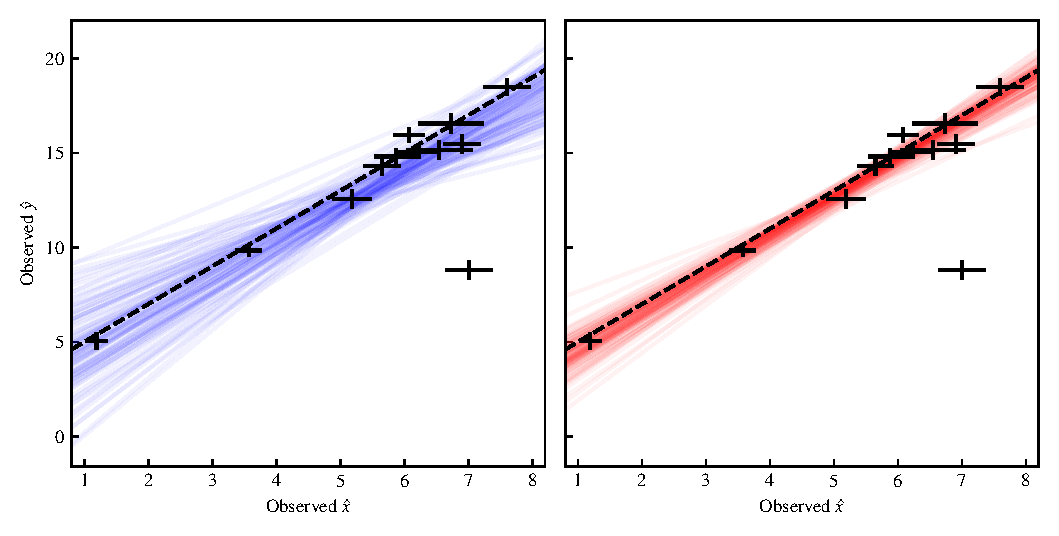
\includegraphics[width=\linewidth]{graphics/fixed/regression_outlier.pdf}
    \caption{100 draws from the posterior of regression lines from
    the normal model (left panel, blue) and $t$-cup (right panel, red). The
    dataset is illustrated by the black points, with the ground-truth regression
    line illustrated by the black dashed line.}
    \label{fig:results.outlier.regression}
\end{figure*}

\begin{figure}
    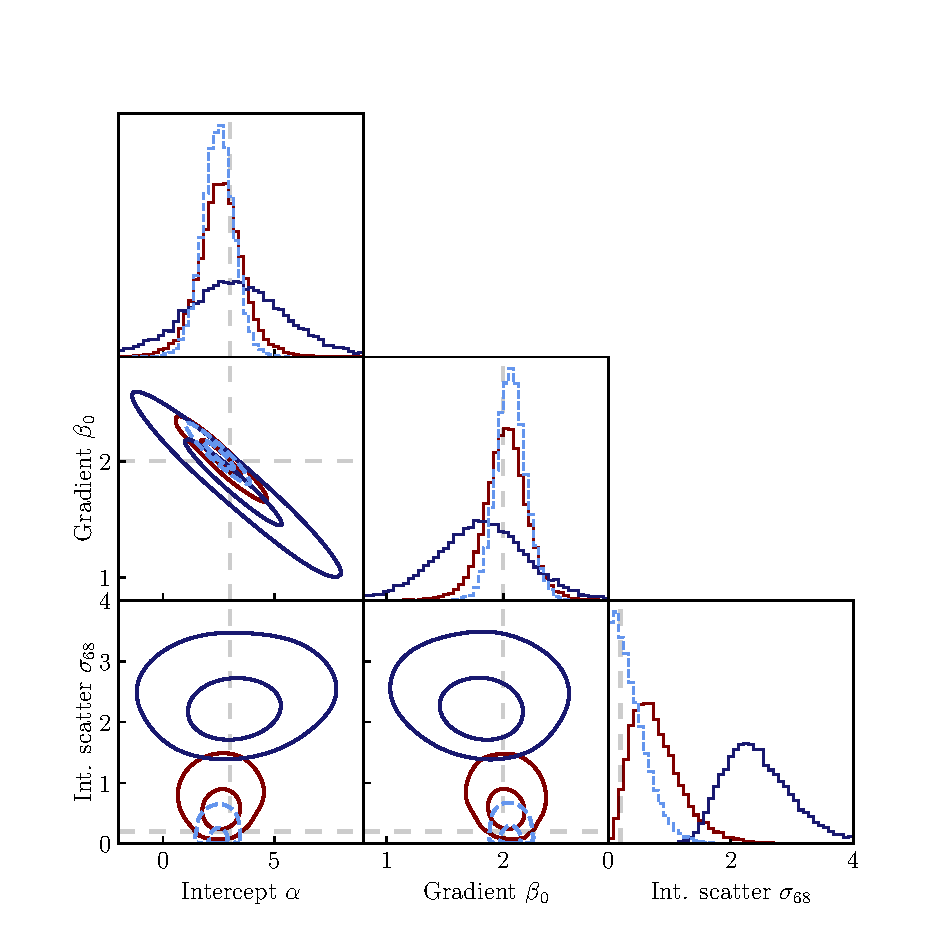
\includegraphics[width=\columnwidth]{graphics/fixed/corner_outlier_ncup.pdf}
    \caption{The posterior for each of the regression coefficients under the
    normal model with the outlier included (dark blue, solid) and excluded
    (light blue, dashed), and for $t$-cup with the outlier included (dark red,
    solid). Ground-truth values are indicated by the black dashed lines.}
    \label{fig:results.outlier.corner}
\end{figure}

\begin{figure}
    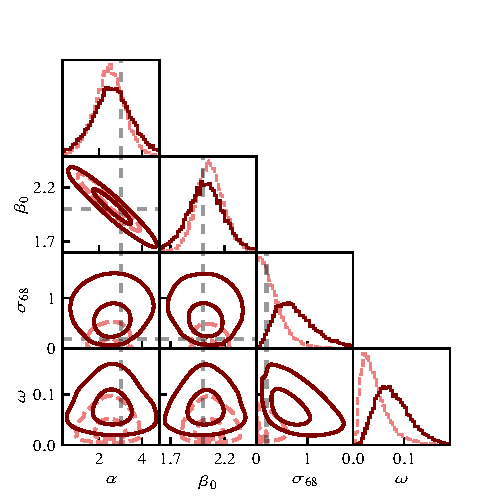
\includegraphics[width=\columnwidth]{graphics/fixed/corner_outlier_tcup.pdf}
    \caption{The posterior for each of the regression coefficients and the shape
    parameter $\nu$ under the $t$-cup model with the outlier included (dark red,
    solid) and excluded (light red, dashed). Ground-truth values are indicated
    by the black dashed lines.}
    \label{fig:results.outlier.tcup}
\end{figure}

Figure \ref{fig:results.outlier.regression} illustrates how the estimates for
the true parameter models are biased in the normal model, but less affected in
the $t$-cup model.

In Figure \ref{fig:results.outlier.corner}, we compare the constraints on
parameters derived under the normal model (including and excluding the outlier
from the dataset), and the $t$-cup model (including the outlier only). The
constraints from the $t$-cup model including the outlier are consistent with
those derived under the normal model when the outlier is excluded, obviating the
need to remove the outlier manually. While this outlier is particularly extreme,
this example illustrates the utility of the $t$-cup model in datasets with
outliers.

For completeness, in Figure \ref{fig:results.outlier.tcup} we illustrate that
the $t$-cup model recovers consistent constraints regardless of whether the
outlier is included or excluded.

\begin{figure*}
    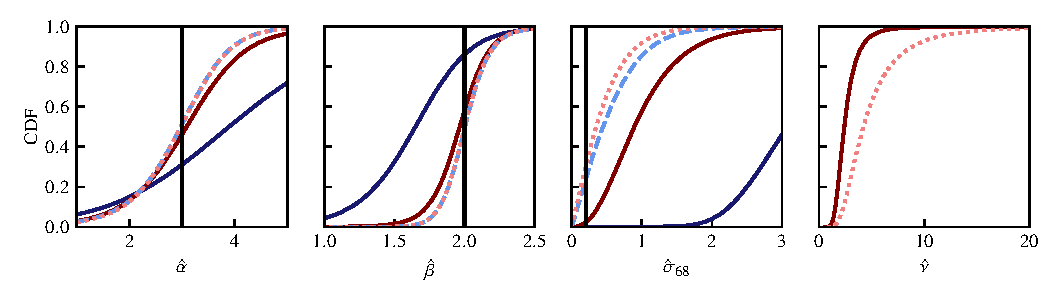
\includegraphics[
        width=\textwidth,
        trim={0 0.3cm 0 0},
        clip
    ]{graphics/fixed/normal_cdf.pdf}
    \caption{The combined cumulative distribution function of the regression
    parameters for 400 normal datasets with an outlier under the normal model
    (dark blue, solid) and $t$-cup model (dark red, solid), and with the outlier
    removed for the normal model (light blue, dashed) and $t$-cup model (light
    red, dashed).}
    \label{fig:results.outlier.map}
\end{figure*}

We then generated 400 datasets using the same procedure, and combined posterior
samples from each run to build an effective cumulative distribution function
across all runs for both the normal model and for $t$-cup. The results
(illustrated in Figure \ref{fig:results.outlier.map}) indicate that constraints
under $t$-cup are significantly less biased than those calculated under the
normal model.

% We also compared the 95\% highest-posterior density credible
% intervals for each parameter, finding that the true parameter value was
% contained within the interval for $x$\% of parameters and runs.
% 
% \begin{table}
% 	\centering
% 	\caption{Percentage of 95\% highest posterior density credible intervals
% 	containing the true parameter value across 400 runs (excluding runs with
% 	$\hat{R} > 1.1$).}
% 	\label{tab:real-world.kelly.params}
% 	\begin{tabular}{lcccc} % four columns, alignment for each
%                                & \multicolumn{2}{c}{Outlier excluded} & \multicolumn{2}{c}{Outlier included} \\
%                                & $n$-cup   & $t$-cup & $n$-cup & $t$-cup       \\
%     Intercept $\alpha$         & 96.7\% & 97.5\% & 100\% & 99.4\% \\
%     Slope $\beta$              & 97.5\% & 97.7\% & 96.7\% & 99.7\% \\
%     Int. scatter $\sigma_{68}$ & 97.5\% & 97.7\% & 0\% & 75.8\% \\
% \end{tabular}
% \end{table}

\subsection{Two-dimensional normal mixture model with outliers}
\label{sec:results.gmm}

This test is designed to further explore how $t$-cup performs when the model is
misspecified. In this case, we are looking at a normally-distributed population
which has a 10\% contamination rate with another normally-distributed population
of the same mean but 10 times the standard deviation. Equivalently, this test
can be thought of as investigating how the model performs when there is a
significant fraction of outliers.

The intrinsic scatter distribution $\mathcal P_{\rm int}$ is a mixture of two
normal distributions with zero mean; 90\% of points are drawn from a core
distribution with standard deviation $\sigma_\textrm{int}$, and 10\% of points
are drawn from an outlier distribution with standard deviation $10
\sigma_\textrm{int}$. The observation distribution $\mathcal P_{\rm obs}$ is a
normal distribution. For fixed-value tests, the true values of the regression
parameters were fixed to $(\alpha, \beta_0, \beta_1, \sigma_{\rm int}) = (2,
3, 1, 0.4)$. The full generative model for the fixed-value tests is given in
Appendix \ref{sec:data-models.gmm}.

The results (see Figure \ref{fig:results.gmm.corner}) show that, while the
constraints from the normal model are significantly biased for this generative
distribution, $t$-cup is able to recover the correct parameter values.

\begin{figure}
    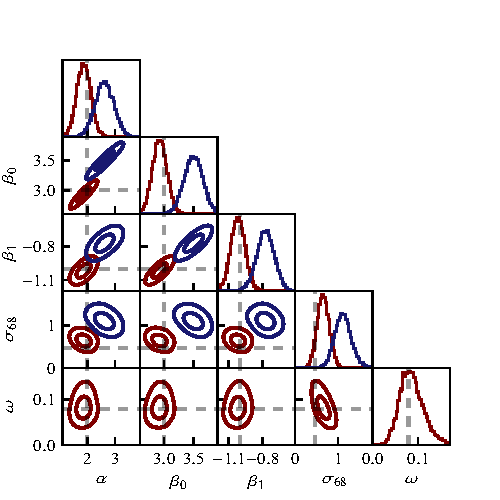
\includegraphics[width=\columnwidth]{graphics/fixed/corner_gaussian_mix.pdf}
    \caption{The posterior for each of the regression coefficients and the
    outlier fraction $\omega$ for the normal mixture model dataset, with
    ground-truth values indicated by the grey dashed lines.}
    \label{fig:results.gmm.corner}
\end{figure}

% \begin{figure*}
%     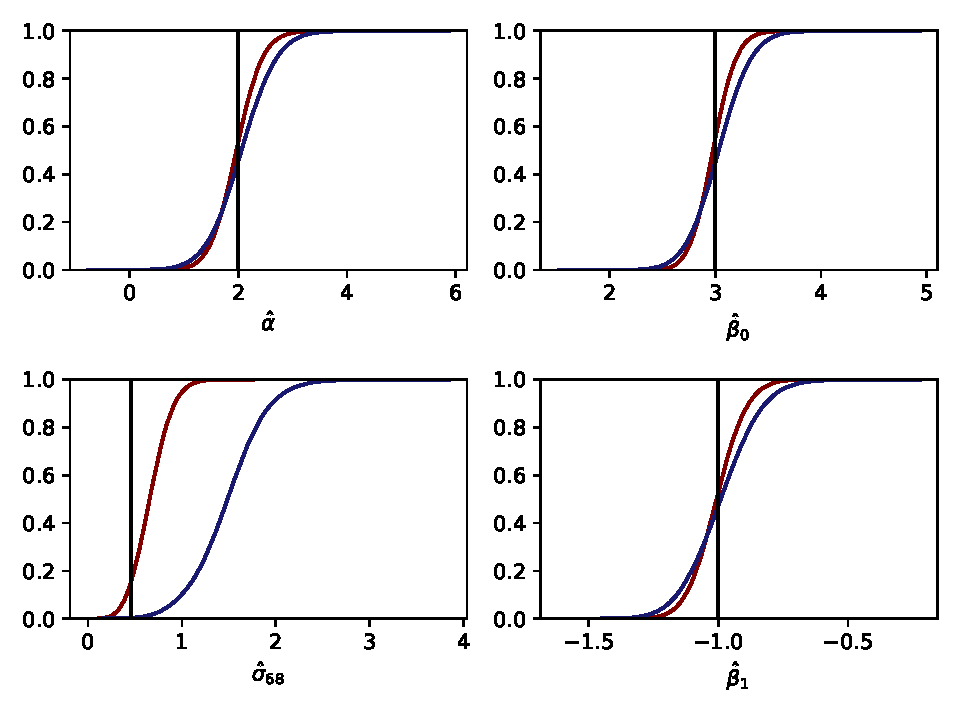
\includegraphics[width=\textwidth, trim={0 0.3cm 0 0}, clip]{graphics/fixed/gaussian_mix_cdf.pdf}
%     \caption{The combined cumulative distribution function of the regression
%     parameters for 400 Gaussian mixture model datasets under the normal model
%     (blue) and $t$-cup model (red).}
%     \label{fig:results.gmm.map}
% \end{figure*}

\subsection{Laplace-distributed data}
\label{sec:results.laplace}

As the underlying sampling distributions can never be known with certainty it is
important to test the method on data generated from a distribution that does not
fall into the family of $t$-distributions (and has a high outlier fraction).
Here we use a Laplace distribution as $\mathcal P_{\rm int}$, giving another
example of performance under explicit model mis-specification.

We generate $N = 25$ datapoints from a model with Laplacian intrinsic scatter
(i.e.\ $\mathcal P_{\rm int} = \mathrm{Laplace}$) and normally distributed observation
noise (i.e.\ $\mathcal P_{\rm obs} = \mathcal N$). For the fixed-value tests, we
set $(\alpha, \beta, \sigma_{\rm int}) = (-1, 0.8, 0.2)$. The full
generative model can be found in Appendix \ref{sec:data-models.laplace}.

\begin{figure}
    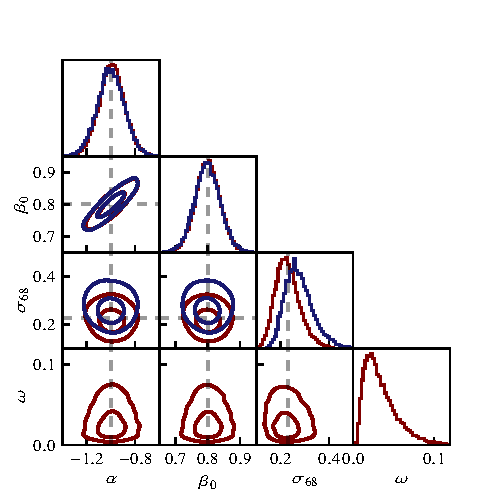
\includegraphics[width=\columnwidth]{graphics/fixed/corner_laplace.pdf}
    \caption{The posterior for each of the regression coefficients and the shape
    parameter $\nu$ for the Laplace-distributed dataset, with ground-truth
    values indicated by the black dashed lines.}
    \label{fig:results.laplace.corner}
\end{figure}

As we can see in Figure \ref{fig:results.laplace.corner}, while both $n$-cup and
$t$-cup successfully recover the gradient and intercept that were used to
generate the dataset, $n$-cup overpredicts the true intrinsic scatter when
$t$-cup constrains it accurately. To confirm this, we generated 400 datasets
using the same procedure, and analysed each with both $n$-cup and $t$-cup. The
results (illustrated in Figure \ref{fig:results.laplace.map}) show the same
pattern -- that $t$-cup is able to accurately constrain the intrinsic scatter,
while the estimate from the normal model is biased high.

\begin{figure*}
    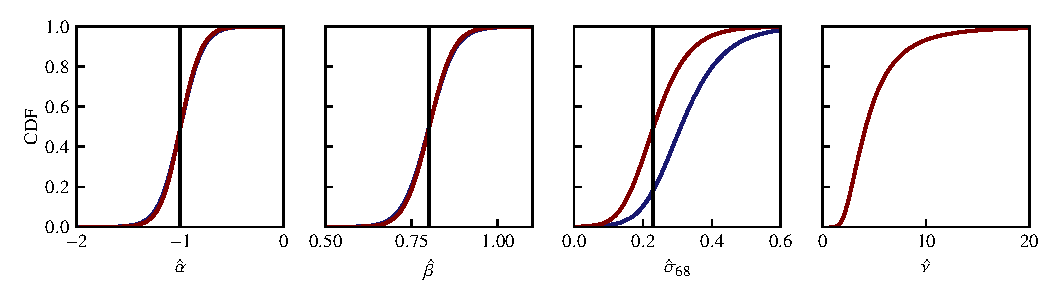
\includegraphics[width=\textwidth, trim={0 0.3cm 0 0}, clip]{graphics/fixed/laplace_cdf.pdf}
    \caption{The combined cumulative distribution function of the regression
    parameters for 400 Laplace datasets under the normal model
    (blue) and $t$-cup model (red).}
    \label{fig:results.laplace.map}
\end{figure*}

\section{Demonstration on real data}
\label{sec:real-world}

Having seen $t$-cup's performance on simulated data in the previous section, we
now compare the performance of the $t$-cup model with a generic astronomical
Bayesian linear regression model \citep[\textsc{linmix\_err};][]{Kelly:2007} and
a tailored approach using $t$-distributions \citep{Park:2017}.

\subsection{\textsc{linmix\_err}}

We use the same dataset that is used in Section 8 of \citet{Kelly:2007} -- a
dataset of $N = 39$ quasars with measured Eddington ratio $L / L_{\text{Edd}}$
and X-ray spectral index $\Gamma$. Performance is compared with a Python
implementation\footnotemark of the original \textsc{linmix\_err} paper proposed
by \citeauthor{Kelly:2007} -- see Figure \ref{fig:real-world.kelly.regression}.

\footnotetext{\url{https://github.com/jmeyers314/linmix}}

\begin{figure*}
    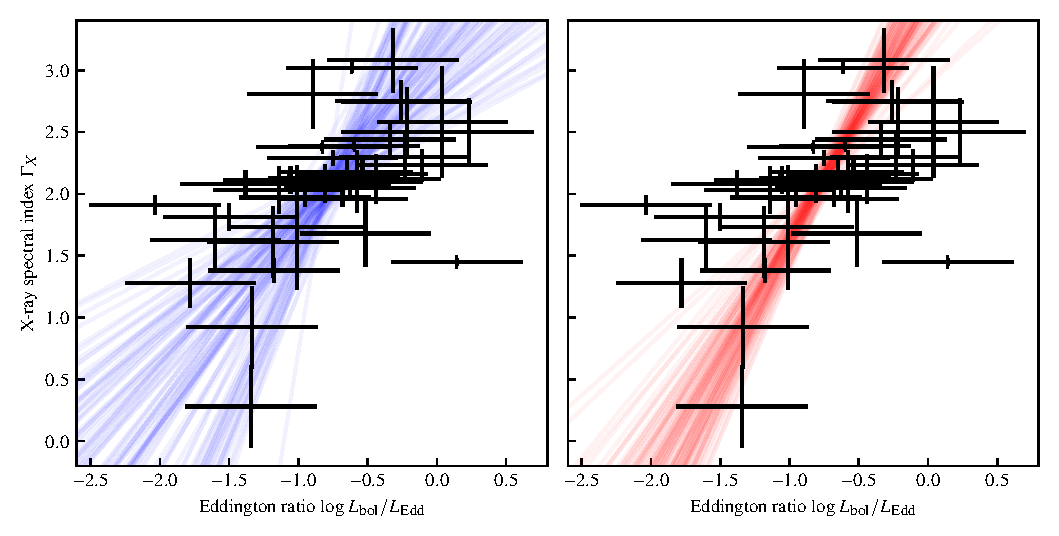
\includegraphics[width=\linewidth]{graphics/real/regression_kelly.pdf}
    \caption{100 draws from the posterior of regression lines from
    \textsc{linmix\_err} (left panel, blue) and $t$-cup (right panel, red) for
    the \citet{Kelly:2007} dataset.}
    \label{fig:real-world.kelly.regression}
\end{figure*}

\begin{table}
	\centering
	\caption{Estimates for the intercept, slope, and intrinsic scatter inferred for
	the relationship between Eddington ratio $L / L_{\text{Edd}}$ and X-ray
	spectral index $\Gamma$ for the sample of quasars analysed by
	\citet{Kelly:2007}. The parameter estimates reported in \citet{Kelly:2007} are
	the posterior median and ``a robust estimate of the standard deviation''; for
	linmix and $t$-cup, we report the posterior median and an estimate of the
	standard deviation as $\sigma = 1.4826 \, \text{MAD}$, where MAD is the median
	absolute deviation.}
	\label{tab:real-world.kelly.params}
	\begin{tabular}{lccc} % four columns, alignment for each
                               & \citet{Kelly:2007} & linmix   & $t$-cup       \\
    Intercept $\alpha$         & 3.12 $\pm$ 0.41 & 3.18 $\pm$ 0.48 & 3.62 $\pm$ 0.26 \\
    Slope $\beta$              & 1.35 $\pm$ 0.54 & 1.40 $\pm$ 0.60 & 2.00 $\pm$ 0.33 \\
    Int. scatter $\sigma_{68}$ & 0.26 $\pm$ 0.11 & 0.25 $\pm$ 0.12 & 0.08 $\pm$ 0.07 \\
    Outlier fraction $\omega$  &      ---      &      ---      & 0.04 $\pm$ 0.03 \\
\end{tabular}
\end{table}

While the parameter estimates are broadly consistent (see Table
\ref{tab:real-world.kelly.params}), the posterior distributions in Figure
\ref{fig:real-world.kelly.corner} can be seen to differ, with the posterior
inferred by \textsc{linmix} being more diffuse than that inferred by $t$-cup.
The tighter constraints of $t$-cup suggest that the inference presented by
\citet{Kelly:2007} may be biased by the enforced assumption of
normally-distributed data, which may not be accurate. The explicit assumption of
normality in \textsc{linmix} is in tension with the outlier fraction estimated
by $t$-cup (68\% CI $\omega = 0.05$\raisebox{0.5ex}{\tiny$^{+0.04}_{-0.01}$}).
This showcases that analysing data with robust procedures gives materially
different answers on real-world data, and highlights the importance of carefully
considering the implications when assuming normality.

\begin{figure}
    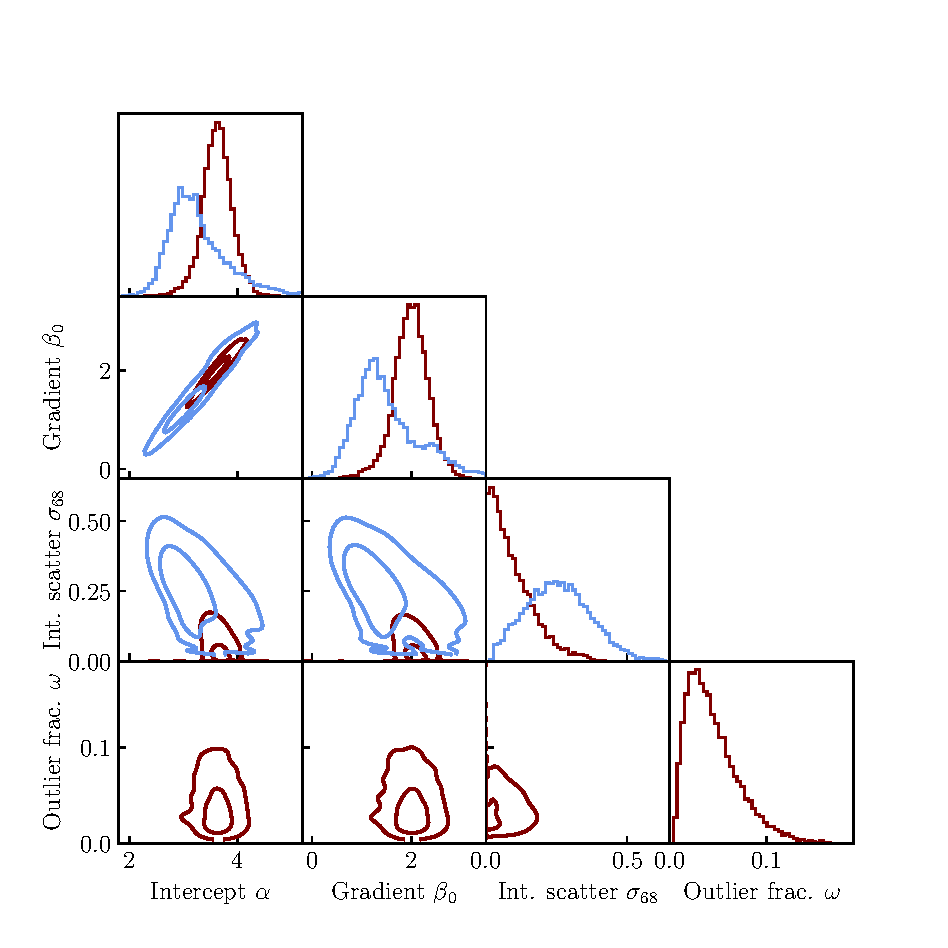
\includegraphics[width=\columnwidth]{graphics/real/corner_kelly.pdf}
    \caption{The posterior distributions for the data from \citet{Kelly:2007}
    under the linmix (blue) and $t$-cup (red) models.}
    \label{fig:real-world.kelly.corner}
\end{figure}

\subsection[Park et al. (2017)]{\citet{Park:2017}}

This dataset consists of $N = 31$ AGN with reverberation-mapped mass estimates,
$M_{\text{BH}}$, \ion{C}{iv} emission line width, $\Delta V$, and continuum
luminosities, $\lambda L_{\lambda}$. Three different \ion{C}{iv} line width
measurements are compared in \citet{Park:2017}: the full-width at half maximum
(FWHM), the line dispersion, $\sigma_l$, and the median absolute deviation. This
dataset is used to fit the regression relation
\begin{equation}
    \log_{10}\!\left( \frac{M_{\text{BH}}}{10^8 M_\odot} \right)\! =
        \alpha +
        \beta \log_{10}\! \left( \frac{\lambda L_{\lambda}}{10^{44} \text{erg s}^{-1}} \right) +
        \gamma \log_{10}\!\left( \frac{\Delta V}{10^3 \text{km s}^{-1}} \right).
        \label{eqn:real-world.park}
\end{equation}
The $t$-cup posterior for parameters $\alpha$, $\beta$ and $\gamma$, as well as
intrinsic scatter $\sigma_{68}$ and shape parameter $\nu$, is shown in Figure
\ref{fig:real-world.park.corner}.

The constraints on the intercept, $\alpha$, and slopes, $\beta$ and $\gamma$,
are consistent with those derived by \citet{Park:2017} for all three measures of
emission line width --- see Table \ref{tab:real-world.park.params}.
\citet{Park:2017} predicts a systematically higher intrinsic scatter than that
predicted by $t$-cup, however, these figures cannot be compared directly, as
this may be influenced by different prior choice for $\nu$.

\begin{table*}
	\centering
	\caption{A comparison between the constraints on the parameters in Equation
	\ref{eqn:real-world.park} derived by \citet{Park:2017} and using $t$-cup.}
	\label{tab:real-world.park.params}
	\begin{tabular}{lcc|cc|cc} % seven columns, alignment for each
                          & \multicolumn{2}{c}{FWHM} & \multicolumn{2}{c}{$\sigma_l$} & \multicolumn{2}{c}{MAD} \\
                          & \citet{Park:2017} & $t$-cup & \citet{Park:2017} & $t$-cup & \citet{Park:2017} & $t$-cup \\
    Intercept $\alpha$    & $7.54$\raisebox{0.5ex}{\tiny$^{+0.26}_{-0.27}$} & $7.51$\raisebox{0.5ex}{\tiny$^{+0.22}_{-0.22}$} & $6.90$\raisebox{0.5ex}{\tiny$^{+0.35}_{-0.34}$} & $6.91$\raisebox{0.5ex}{\tiny$^{+0.30}_{-0.31}$} & $7.15$\raisebox{0.5ex}{\tiny$^{+0.24}_{-0.25}$} & $7.15$\raisebox{0.5ex}{\tiny$^{+0.22}_{-0.22}$} \\
    Slope $\beta$         & $0.45$\raisebox{0.5ex}{\tiny$^{+0.08}_{-0.08}$} & $0.43$\raisebox{0.5ex}{\tiny$^{+0.06}_{-0.06}$} & $0.44$\raisebox{0.5ex}{\tiny$^{+0.07}_{-0.07}$} & $0.43$\raisebox{0.5ex}{\tiny$^{+0.05}_{-0.06}$} & $0.42$\raisebox{0.5ex}{\tiny$^{+0.07}_{-0.07}$} & $0.42$\raisebox{0.5ex}{\tiny$^{+0.05}_{-0.06}$} \\
    Slope $\gamma$        & $0.50$\raisebox{0.5ex}{\tiny$^{+0.55}_{-0.53}$} & $0.58$\raisebox{0.5ex}{\tiny$^{+0.44}_{-0.45}$} & $1.66$\raisebox{0.5ex}{\tiny$^{+0.65}_{-0.66}$} & $1.66$\raisebox{0.5ex}{\tiny$^{+0.57}_{-0.58}$} & $1.65$\raisebox{0.5ex}{\tiny$^{+0.61}_{-0.62}$} & $1.65$\raisebox{0.5ex}{\tiny$^{+0.55}_{-0.55}$} \\
    Int. scatter $\sigma$ & $0.16$\raisebox{0.5ex}{\tiny$^{+0.10}_{-0.08}$} & $0.10$\raisebox{0.5ex}{\tiny$^{+0.03}_{-0.10}$} & $0.12$\raisebox{0.5ex}{\tiny$^{+0.09}_{-0.06}$} & $0.08$\raisebox{0.5ex}{\tiny$^{+0.02}_{-0.08}$} & $0.12$\raisebox{0.5ex}{\tiny$^{+0.09}_{-0.06}$} & $0.07$\raisebox{0.5ex}{\tiny$^{+0.02}_{-0.07}$} \\
    \end{tabular}
\end{table*}

\begin{figure}
    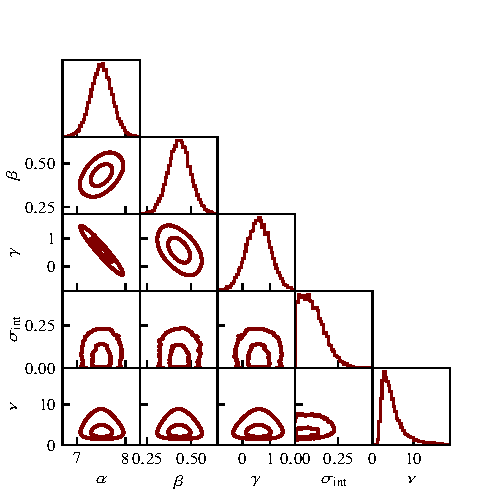
\includegraphics[width=\columnwidth]{graphics/real/corner_park_fwhm.pdf}
    \caption{The posterior distributions for the data from \citet{Park:2017}
    under the $t$-cup model. {\color{red} This figure
    needs updating with param names to match Park.}}
    \label{fig:real-world.park.corner}
\end{figure}

\section{Conclusions}
\label{sec:conclusion}

We have presented a general-purpose approach to linear regression, implemented
as $t$-cup, that is robust to model mis-specification, with a model laid out in
Section \ref{sec:formalism}. In Section \ref{sec:results}, we demonstrated that
the model recovers constraints consistent with those used to generate the
datasets, including in cases where there is a mismatch between the generative
model used to create the dataset and our regression model. In Section
\ref{sec:real-world}, we compared the method to \citet{Kelly:2007, Park:2017} on
real-world data, illustrating that the models derive consistent constraints.

It may be fruitful to re-examine some of the priors assumed in the $t$-cup
model; while we focused on producing a model that was applicable to a large
range of datasets, $t$-cup predicted lower intrinsic scatter than both
\citet{Kelly:2007} and \citet{Park:2017}. While results between the three are
not directly comparable as a result of the different assumptions in each model,
this difference could suggest that the prior on $\sigma_{68}$ has too much
density near $\sigma_{68} = 0$. In addition, setting the prior on
$\{\mathbf{x}_i\}$ using extreme deconvolution, while effective, is not
theoretically motivated; a prior similar to that presented in
\citet{Bartlett:2023} may be more appropriate in this case.

In our next paper, we will apply the robust inference techniques presented here
to exploring the single-epoch mass estimators used in estimating the masses of
high-redshift quasars. 

\section*{Acknowledgements}

The authors would like to thank Stephen Feeney, Boris Leistedt, Justin Alsing,
Tamas Budavari and Chad Schafer for useful conversations. WM is supported by
STFC grant ST/T506151/1.

%%%%%%%%%%%%%%%%%%%%%%%%%%%%%%%%%%%%%%%%%%%%%%%%%%
\section*{Data Availability}

The data in this paper is sourced from \citet{Kelly:2007, Park:2017}. Scripts to
generate the simulated datasets used to validate the model in Section
\ref{sec:results} are available from the GitHub repository for this paper, at
\url{https://github.com/wm1995/tcup-paper}.

%%%%%%%%%%%%%%%%%%%% REFERENCES %%%%%%%%%%%%%%%%%%

\bibliographystyle{rasti}
\bibliography{references}

%%%%%%%%%%%%%%%%%%%%%%%%%%%%%%%%%%%%%%%%%%%%%%%%%%

%%%%%%%%%%%%%%%%% APPENDICES %%%%%%%%%%%%%%%%%%%%%

\appendix

\section{Prior choice for shape parameter}
\label{sec:t-prior}

As our model relies on Student's $t$-distributions, we review notation and
priors used by previous works and justify our reasoning for our prior choice.
One approach is to adopt a fixed value of $\nu$, which is equivalent to setting
a Dirac delta function prior: a common choice is $\nu = 4$
\citep[e.g.][]{Berger:1994, Gelman:2013}.  Another approach is to adopt a more
flexible approach by allowing $\nu$ to vary \citep[e.g.][]{Juarez:2010,
Gelman:2013, Ding:2014, Park:2017, Feeney:2018}.

We sought a flexible prior for this work that could reduce to a (nearly) normal
distribution, but had sufficient flexibility to accommodate heavy-tailed
distributions as well. Priors meeting this criterion include:
\begin{itemize}
    \item priors of the form $\nu \sim \Gamma(\alpha, \beta)$ for
          some shape parameter, $\alpha$, and rate parameter, $\beta$ -- e.g.
          \citet{Juarez:2010} uses $\left\{\alpha = 2, \beta = 0.1\right\}$;
          \citet{Ding:2014} uses $\left\{\alpha = 1, \beta = 0.1\right\}$
    \item A uniform prior in $\frac1\nu \sim U(0, 1)$ \citep{Gelman:2013}
    \item A uniform prior\footnotemark in distribution peak height relative to a normal
    distribution, $t$, such that
    \begin{equation}
        t \equiv \sqrt{\frac2\nu}\frac{\Gamma\left(\frac{\nu + 1}{2}\right)}{\Gamma\left(\frac{\nu}{2}\right)} \sim U(0, 1).
    \end{equation}
\end{itemize}
These priors, along with the prior we adopted, are illustrated in Figure
\ref{fig:priors.pdf}. The cumulative distribution functions for the priors in
terms of outlier fraction, $\omega$, are illustrated in Figure
\ref{fig:priors.outlier_frac}.

\begin{figure}
	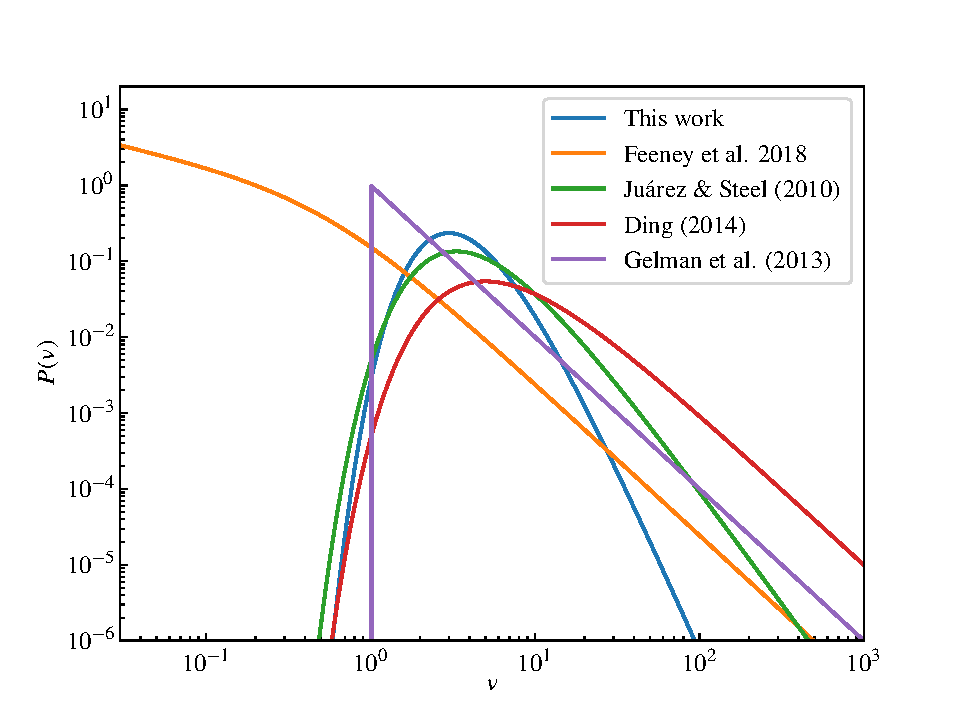
\includegraphics[width=\columnwidth]{graphics/pdf_nu}
    \caption{A selection of different priors on $\nu$ in works that have used
    $t$-distributions.}
    \label{fig:priors.pdf}
\end{figure}

\footnotetext{Strictly, \citet{Feeney:2018} approximate this prior with the closed
form prior on shape parameter, $\nu$, of
\begin{equation*}
    \mathcal P\left(\nu\right) \propto
    \frac{
        \Theta(\nu)
    }{
        \left(
            \left(\frac{\nu}{\nu_0}\right)^{1 / (2 a)}
            + \left(\frac{\nu}{\nu_0}\right)^{2 / a}
        \right)^a
    }
\end{equation*}
where $\Theta(\cdot)$ is the Heaviside step function, and $\nu_0$ and $a$ are
constants with values $\sim 0.55$ and $\sim 1.2$ respectively.
}

When testing different priors, we found that priors with significant density in
the range $0 < \nu < 1$ led to sampling difficulties as $\nu$ approached 0;
these low values of $\nu \sim 0.1$ can correspond to outliers that are more than
20 orders of magnitude larger than $\sigma$. In theory, these unphysical regions
of parameter space ought to be excluded during the process of inference.
However, the use of HMC in such cases can lead to divergences in the sampling
process or inefficient sampling as the sampler struggles with regions of high
curvature --- see the discussion of this phenomenon in \citet{Neal:2003}.

Another option would be to place a prior is on outlier fraction $\omega$. It
could be argued that the term outlier loses its meaning when the majority of a
dataset is composed of so-called ``outliers''; therefore, a natural choice of
prior might be a uniform distribution ranging from the normally-distributed
outlier fraction of $\sim$0.00270 to this ``maximum'' outlier fraction of 0.5,
corresponding to $\nu \sim 0.302$. This still leads to large outliers (some of 8
orders of magnitude for 100 draws from the distribution), which are unphysical
and continue to present difficulties when sampling with HMC.

To limit the number of unphysical outliers, we can instead limit the prior to
consider only distributions that are less heavy-tailed than the Cauchy
distribution --- i.e. all those with $\nu > 1$. This is the approach taken by
\citet{Gelman:2013}, rendering regions of parameter space inaccessible (in the
case of the \citet{Gelman:2013} prior, $\nu = 1$ is the cutoff, which
corresponds to a Cauchy distribution.) On the other hand, the priors used in
\citet{Juarez:2010, Ding:2014, Feeney:2018} have disproportionate prior density
at low values of $\nu$, which corresponds to models with outliers several orders
of magnitude larger than the predicted effect size.

\begin{figure}
	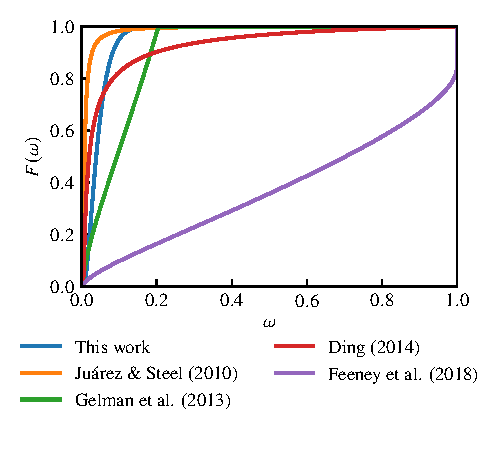
\includegraphics[width=\columnwidth]{graphics/cdf_outlier_frac}
    \caption{The CDF of priors on $\nu$ used in works that have used
    $t$-distributions. The priors are expressed in terms of outlier fraction,
    $\omega$, as defined in Equation \ref{eqn:model.outlier_frac}.}
    \label{fig:priors.outlier_frac}
\end{figure}

In this work, we use the prior
\begin{equation}
    \nu \sim \text{Inv-}\Gamma(4, 15),
\end{equation}
where $\text{Inv-}\Gamma(\alpha, \beta)$ is an inverse gamma distribution with
shape parameter, $\alpha$, and scale parameter, $\beta$.

This prior was chosen for two reasons:
\begin{itemize}
    \item the prior is smooth in $\nu$ with no sharp boundaries (unlike
          \citet{Gelman:2013})
    \item the prior has density at a larger range of outlier fractions $\omega$
          than that in \citet{Juarez:2010} but insignificant density
          at unrealistically high outlier fractions, in contrast with the priors
          in \citet{Ding:2014, Feeney:2018}.
\end{itemize}

\section{Fixed-value calibration data models}
\label{sec:data-models}

Here, we fully specify the dataset models used for fixed-value
calibration tests in Section \ref{sec:results}.

\subsection{\textit{t}-distributed data}
\label{sec:data-models.t}

In Section \ref{sec:results.t}, the fixed-value test datasets have $N = 20$
datapoints drawn from the following distribution:
\begin{align}
    x_i \sim&\; \mathcal N (\mu = 2, \sigma = 2) \\
    y_i \sim&\; t_{3} (\mu = 3 + 2 x_i, \sigma = 0.1 / \sigma_{68}(\nu = 3)) \\
    \log_{10} \sigma_{x, i} \sim&\; \mathcal N (\mu = -1, \sigma = 0.1) \\
    \log_{10} \sigma_{y, i} \sim&\; \mathcal N (\mu = -0.7, \sigma = 0.1) \\
    \hat{x}_i \sim&\; \mathcal N (\mu = x_i, \sigma = \sigma_{x, i}) \\
    \hat{y}_i \sim&\; \mathcal N (\mu = y_i, \sigma = \sigma_{y, i}).
\end{align}

\subsection{Normally-distributed data with an outlier}
\label{sec:data-models.outlier}

In Section \ref{sec:results.outlier}, we generated datasets of $N = 12$ points
using the model:
\begin{alignat}{1}
    x_i& \sim \mathcal N (\mu = 5, \sigma = 3) \\
    y_i& \sim
    \begin{cases}
        \mathcal N (\mu = 3 + 2 x_i - 10, \sigma = 0.2) &
            \text{for the second-largest $x_i$} \\
        \mathcal N (\mu = 3 + 2 x_i, \sigma = 0.2) &
            \text{otherwise} \\
    \end{cases}\\
    \log_{10} \sigma_{x, i}& \sim \mathcal N (\mu = -0.5, \sigma = 0.1) \\
    \log_{10} \sigma_{y, i}& \sim \mathcal N (\mu = -0.3, \sigma = 0.1) \\
    \hat{x}_i& \sim \mathcal N (\mu = x_i, \sigma = \sigma_{x, i}) \\
    \hat{y}_i& \sim \mathcal N (\mu = y_i, \sigma = \sigma_{y, i}).
\end{alignat}

\subsection{Two-dimensional normal mixture model}
\label{sec:data-models.gmm}

We introduce the parameter $O_i$ to indicate whether the $i$th datapoint is
drawn from the core distribution (in which case, $O_i = 0$) or from the outlier
distribution (for which $O_i = 1$).

In Section \ref{sec:results.gmm}, we generated a dataset of $N = 200$ points
using the model:
\begin{alignat}{1}
    \boldsymbol{x}_i& \sim
    \begin{cases}
        \mathcal N \left(
            \mu = \begin{pmatrix} -3 \\ 2 \end{pmatrix},
            \sigma = \begin{pmatrix} 0.5 & -1 \\ -1 & 4 \end{pmatrix}
        \right) &
            1 \leqslant i \leqslant 140 \\
        \mathcal N \left(
            \mu = \begin{pmatrix} -1 \\ -1 \end{pmatrix},
            \sigma = \begin{pmatrix} 1 & 0.2 \\ 0.2 & 0.8 \end{pmatrix}
        \right) &
            140 < i \leqslant 200 \\
    \end{cases}\\
    O_i& \sim \mathrm{Bernoulli}(0.1) \\
    y_i& \sim
    \begin{cases}
        \mathcal N (\mu = 2 + (3, 1)^T \cdot x_i, \sigma = 0.4) &
            O_i = 0 \\
        \mathcal N (\mu = 2 + (3, 1)^T \cdot x_i, \sigma = 4.0) &
            O_i = 1 \\
    \end{cases}\\
    \Sigma_{x, i}& \sim \mathcal W_2 (\boldsymbol{V} = 0.1 \mathbb{I}, n = 3) \\
    \log_{10} \sigma_{y, i}& \sim \mathcal N (\mu = -1, \sigma = 0.1) \\
    \hat{x}_i& \sim \mathcal N (\mu = \boldsymbol{x}_i, \sigma = \Sigma_{x, i}) \\
    \hat{y}_i& \sim \mathcal N (\mu = y_i, \sigma = \sigma_{y, i}),
\end{alignat}
where $\mathcal W_2$ denotes a Wishart distribution over 2x2 matrices and
$\mathbb{I}$ denotes the 2x2 identity matrix.

\subsection{Laplace-distributed data}
\label{sec:data-models.laplace}

In Section \ref{sec:results.laplace}, we generate $N = 25$ datapoints under the
following model:
\begin{eqnarray}
    x_i &\sim& \mathcal U (-5, 5) \\
    y_i &\sim& \mathrm{Laplace} (\mu = -1 + 0.8 x_i, b = 0.2) \\
    \log_{10} \sigma_{x, i} &\sim& \mathcal N (\mu = -1, \sigma = 0.1) \\
    \log_{10} \sigma_{y, i} &\sim& \mathcal N (\mu = -1, \sigma = 0.1) \\
    \hat{x}_i &\sim& \mathcal N (\mu = x_i, \sigma = \sigma_{x, i}) \\
    \hat{y}_i &\sim& \mathcal N (\mu = y_i, \sigma = \sigma_{y, i}).
\end{eqnarray}

% \subsection{Log-normal distributed data}
% \label{sec:data-models.lognormal}

% We generate $N = 25$ datapoints under the following model:
% \begin{eqnarray}
%     x_i &\sim& \mathcal U (-5, 5) \\
%     \log_{10} y_i &\sim& \mathcal N (\mu = \log_{10} (4 + 8 x_i), \sigma = 0.2) \\
%     \log_{10} \sigma_{x, i} &\sim& \mathcal N (\mu = -1, \sigma = 0.1) \\
%     \log_{10} \sigma_{y, i} &\sim& \mathcal N (\mu = -1, \sigma = 0.1) \\
%     \hat{x}_i &\sim& \mathcal N (\mu = x_i, \sigma = \sigma_{x, i}) \\
%     \hat{y}_i &\sim& \mathcal N (\mu = y_i, \sigma = \sigma_{y, i}).
% \end{eqnarray}


%%%%%%%%%%%%%%%%%%%%%%%%%%%%%%%%%%%%%%%%%%%%%%%%%%


% Don't change these lines
\bsp	% typesetting comment
\label{lastpage}
\end{document}

% End of rasti_template.tex
